%-+- coding:UTF-8  -+-
%华北电力大学本科毕业设计(论文)模版1_2.tex
%作者:孙霖,华北电力大学信息1502
%历史记录
%2019/04/11         SunLIn          建立模板并边学习
%2019/04/14         SunLIn          第一次优化
%2019/04/17          SunLIn         补充内容
%macOS/Linux计算字数(终端运行) ./texcount.pl ~/Desktop/毕业设计/02-稿件/华北电力大学本科毕业设计(论文)模版1_2/华北电力大学本科毕业设计(论文)模版1_2.tex(根据自己定义的路径)
\documentclass[UTF8,a4paper]{ctexrep}
\usepackage{geometry}
\usepackage{fancyhdr}
\usepackage{graphicx}
\usepackage{titlesec}
\usepackage{fontspec}
\usepackage[titles]{tocloft}
\usepackage{caption}
\usepackage{booktabs}
\usepackage{tabularx}
\usepackage{setspace}
%防止报错--重定义
\makeatletter
\let\c@lofdepth\relax
\let\c@lotdepth\relax
\makeatother
\usepackage{subfigure}
%防止报错--重定义
%%%%字体字号设置
% 小四, 1.5倍行距
\newcommand{\xiaosi}{\fontsize{12pt}{18pt}\selectfont}            
% 四号, 1.5 倍行距
\newcommand{\sihao}{\fontsize{14pt}{21pt}\selectfont}            
\setmainfont{Times New Roman}
\fontsize{12pt}{18pt}
\selectfont
%%%%文档整体设置
%%设置页眉页脚
%\fancypagestyle{plain}{%

%\fancyhf{} % 清空当前设置

% 设置页眉 (head)
\fancyhead[L,R]{}
\fancyhead[C]{华北电力大学本科毕业设计(论文)}
\pagestyle{fancy}
%%标题整体设置
%\titleformat{\chapter}{\centering}{第\,\thechapter\,章}{1em}{}
\titleformat{\section}{\raggedright\zihao{3}\heiti}{\thesection \quad}{0pt}{}
\titleformat{\subsection}{\raggedright\zihao{-3}\heiti}{\thesubsection }{0pt}{}
%%
%图片编号
\renewcommand {\thetable} {\thechapter{}-\arabic{table}} 
\renewcommand {\thefigure} {\thechapter{}-\arabic{figure}}
%%纸张规格为A4 ;版面上空2.5cm,下空2cm,左空2.5 cm,右空2 cm(左装订)
\geometry{
  left=2.5cm,
  right=2cm,
  top=2.5cm, 
  bottom=2cm,
}
%参考文献方式
\bibliographystyle{plain}
\begin{document}
%%初始配置
%图片题注
%\captionsetup[figure]{name={图-}}
%%插入封面 
%%/***************************************************************/
%%摘要页
\zihao{-4}\songti
%%黑体四号,摘要之间空4个字符
%页码计数器
\chapter*{摘\qquad 要}{\heiti\zihao{4}}
\addcontentsline{toc}{chapter}{摘\qquad 要}
\pagenumbering{Roman}
%%空一行宋体小四号
空一行宋体小四号

\noindent
\qquad 摘要内容,首行空2字符,字数400字左右

%%用宋体小四号,首行空2字符,字数400字左右。
%空一行宋体小四号
%%添加关键词关键词三个字左顶格,用宋体小四号加粗,3-5个关键词用宋体小四号,
%%词于词之间用逗号隔开,最后一个词不加任何标点符号。

\noindent
关键词:
\clearpage
%%/***************************************************************/
%%ABSTRACT

%Times New Roman字体、小四加粗
\chapter*{\textbf{ABSTRACT}}{\zihao{-4}\bf}
\addcontentsline{toc}{chapter}{ABSTRACT}
%空一行,Times New Roman字体、小四号
%Times New Roman字体、小四,首行空4个字母

\qquad  ABSTRACT With English

%关键词左顶格,Times New Roman字体、小四加粗,3-5个关键词Times New Roman字体、小四号,
%词于词之间用逗号隔开,最后一个词不加任何标点符号。
KEYWORDS:
\newpage
%%/***************************************************************/
%%目录
%%%%%给第一级标题加点
\renewcommand{\cftdot}{$\cdot$}
\renewcommand{\cftdotsep}{1.5}
\setlength{\cftbeforechapskip}{10pt}

\renewcommand{\cftchapleader}{\cftdotfill{\cftchapdotsep}}
\renewcommand{\cftchapdotsep}{\cftdotsep}
\makeatletter
\renewcommand{\numberline}[1]{%
\settowidth\@tempdimb{#1\hspace{0.5em}}%
\ifdim\@tempdima<\@tempdimb%
  \@tempdima=\@tempdimb%
\fi%
\hb@xt@\@tempdima{\@cftbsnum #1\@cftasnum\hfil}\@cftasnumb}
\makeatother
%%%%%给第一级标题加点
%黑体四号,目录两个字之间空4个字
\pagenumbering{arabic}
\renewcommand\contentsname{目\qquad 录}
\tableofcontents
%\tableofcontents{section}{\songti\zihao{-4}}
%\tableofcontents{subsection}{\songti\zihao{-4}}
%%/***************************************************************/
%%图目录
\renewcommand*{\listfigurename}{图目录}
\listoffigures
\addcontentsline{toc}{chapter}{图目录}
%%/***************************************************************/
%%表目录
\renewcommand*{\listtablename}{表目录}
\listoftables
\addcontentsline{toc}{chapter}{表目录}

%黑体小四号:摘要、ABSTRACT、一级标题
%宋体小四号:二级三级
\clearpage
\pagenumbering{arabic}

%%/***************************************************************/
%%正文
\zihao{-4}\songti
%%/***************************************************************/
%%第一章
\chapter{绪论}{\heiti\zihao{-2}}
\thispagestyle{fancy}

  \section{课题背景}
  这里引用文献\cite{REF_13浅探应急通信保障中无线自组网技术的应用}。
  \section{国内外研究现状}
    \subsection{电能质量监测国内外研究现状}
    \subsection{无线自组网的国内外研究现状}
    \thispagestyle{fancy}

  \section{本文研究内容和结构组织}

%%/***************************************************************/
%%/***************************************************************/
%%/***************************************************************/
%%第二章
\clearpage
\chapter{总体设计}{\heiti\zihao{-2}}
\thispagestyle{fancy}
\section{相关技术介绍}
  \subsection{STM32嵌入式程序设计}
  这里插入图片。
  %%图片2-1插入

  \begin{figure}[ht]
  \centering
  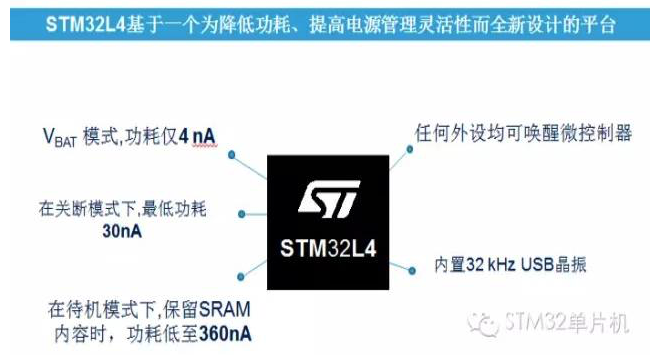
\includegraphics[width=15cm]{Picture/图2-1STM32L4系列.png}
  \caption{STM32L4系列}
  \label{fig:STM32L4系列}
  \end{figure}


  %此处放软件编程
  %%/***************************************************************/
  \subsection{无线自组网}
  %%图片2-2插入
  表格插入

  \begin{table}[ht]
    \centering
    \caption{网路设备各层及所需确定的参数表}
    \begin{tabular}{c|c}
      \toprule
      网络设备  & 配置参数 \\
      \hline
      MAC     &   MAC协议选择及参数\\
      \hline
      信道    &    传输损耗、延时等参数\\
      \hline
      物理层    &   无线网卡(硬件设备及驱动)、工作频率、发射频率、接收门限、噪声等\\
      \bottomrule
    \end{tabular}
  \end{table}
  
\begin{figure}[ht]
  \centering
  \subfigure[蜂窝移动通信拓扑示意图]
  {
    \begin{minipage}{6cm}
    \centering
    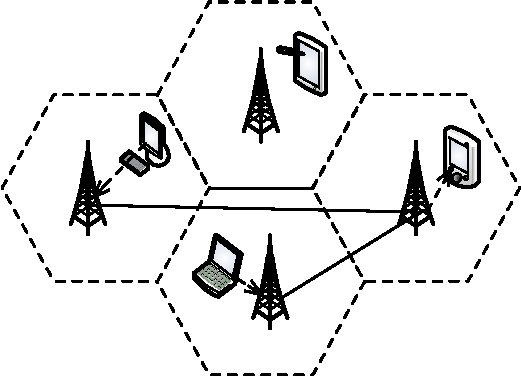
\includegraphics[width=6cm]{Picture/图2-2-1蜂窝移动通信拓扑示意图.pdf}
    \end{minipage}
  }
  \subfigure[无线自组网网络拓扑结构图]
  {
    \begin{minipage}{6cm}
      \centering
      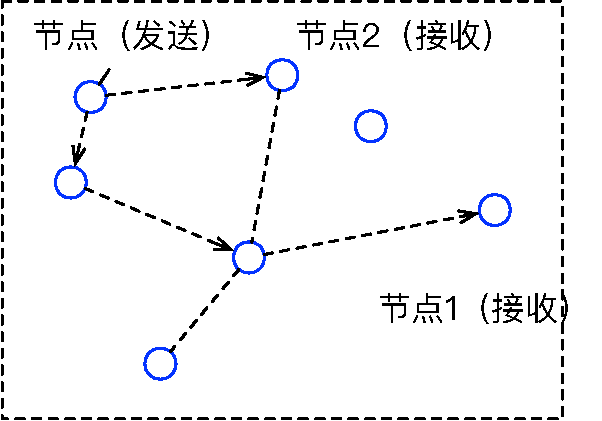
\includegraphics[width=6cm]{Picture/图2-2-2无线自组网网络拓扑结构图.pdf}
      \end{minipage}
  }
  \caption{蜂窝移动通信拓扑示意图和无线自组织网络网络拓扑示意图}
  \label{fig:蜂窝移动通信拓扑示意图和无线自组织网络网络拓扑示意图}
\end{figure}
  %%/***************************************************************/
  \subsection{神经网络}
  %%/***************************************************************/
  \subsection{电能质量分析}
%%/***************************************************************/
%%/***************************************************************/
\section{系统总体架构设计}

%%/***************************************************************/
%%第三章
\chapter{仿真结果与分析}{\heiti\zihao{-2}}
\thispagestyle{fancy}
\section{ns-3网络模拟器与仿真结果与分析}
\section{基于神经网络的电能质量信息处理结果与分析}
%%/***************************************************************/
%%第四章
\chapter{总结与展望}{\heiti\zihao{-2}}
\thispagestyle{fancy}
\section{总结}
\section{展望}
\clearpage
%重新用阿拉伯文字记页码数
%%/***************************************************************/
%%参考文献
\pagenumbering{arabic}
%\chapter*{参考文献}{\heiti\zihao{-2}}
\bibliography{参考文献}
\addcontentsline{toc}{chapter}{参考文献}
\thispagestyle{fancy}
%%/***************************************************************/
%%附录
\chapter*{附\qquad 录}{\heiti\zihao{-2}}
\addcontentsline{toc}{chapter}{附\qquad 录}
\thispagestyle{fancy}
论文的附录依次按附录A,附录B 等进行编号。附录内容的书写格式按毕业设计(论文)的正文规定格式书写。
%%/***************************************************************/
%%致谢
\chapter*{致\qquad 谢}{\heiti\zihao{-2}}
\addcontentsline{toc}{chapter}{致\qquad 谢}
\thispagestyle{fancy}
对曾经给予本人顺利完成毕业设计(论文)而提供各类帮助、指导,以及协助完成该项研究工作的单位和个人表示感谢。


\end{document}